\documentclass[a4paper,12pt]{article} % тип документа

%  Русский язык
\usepackage[T2A]{fontenc}			% кодировка
\usepackage[utf8]{inputenc}			% кодировка исходного текста
\usepackage[english,russian]{babel}	% локализация и переносы

\usepackage{graphicx, scalerel}               % импорт изображений
\usepackage{wrapfig}                % обтекаемые изображения
\graphicspath{{pictures/}}          % обращение к подкаталогу с изображениями
\usepackage[14pt]{extsizes}         % для того чтобы задать нестандартный 14-ый размер шрифта
\usepackage[warn]{mathtext}         % русский язык в формулах
\usepackage{indentfirst}            % indent first
\usepackage[margin = 25mm]{geometry}% отступы полей
\usepackage[table,xcdraw]{xcolor}   % таблицы
\usepackage{amsmath,amsfonts,amssymb,amsthm,mathtools} % Математика
\usepackage{wasysym}                % ???
\usepackage{upgreek}                % ???  
\usepackage{caption}
\usepackage{multirow}
\captionsetup{labelsep=period}
\usepackage[font=small,labelfont=bf]{caption}
\usepackage{gensymb} % degree symbol
\usepackage{tikz}
\usetikzlibrary{positioning}


\begin{document}
	
	
	\begin{center}
		
		\textbf{НАЦИОНАЛЬНЫЙ ИССЛЕДОВАТЕЛЬСКИЙ УНИВЕРСИТЕТ \\ <<МОСКОВСКИЙ ФИЗИКО-ТЕХНИЧЕСКИЙ ИНСТИТУТ>>}
		\vspace{13ex}
		
		\textbf{Лабораторная работа 5.1.2\\ <<Исследование эффекта Комптона>>}
		\vspace{40ex}
		
		\normalsize{Шумаков Иван Игоревич \\ студент группы Б01-009\\ 3 курс ФРКТ\\}
	\end{center}
	
	\vfill 
	
	\begin{center}
		г. Долгопрудный\\ 
		2022 г.
	\end{center}
	
	
	\thispagestyle{empty} % выключаем отображение номера для этой страницы
	\newpage


	\textbf{Цель работы:} Исследовать энергетический спектр рассеянных на графите $\gamma$-квантов.\par
  \textbf{В работе используются:} Источник $\gamma$-лучей, рассеиватель из графита, детектор излучения.\par
    
	\section{Теоретические сведения}

    Пусть на покоящийся электрон (энергия покоя $mc^2$) налетает $\gamma$-квант с начальной энергией $\hbar \omega_0$.
    После соударения электрон приобретает энергию $\gamma mc^2$ и импульс $\gamma mv$, а $\gamma$-квант рассеивается на некотрый угол $\theta$ по отношению к начальному направлению с новой энергией $\hbar \omega_1$. 
    Из законов сохранения импульса и энергии можно получить, что разница между длинами волн падающего и рассенного $\gamma$-квантов
    \begin{equation}\label{1}
      \Delta \lambda = \lambda_1 - \lambda_0 = \dfrac{h}{mc} (1-\cos \theta).
    \end{equation}
    В наличии этой разницы и заключается эффект Комптона. 
    Для дальнейшего применения полезно будет представить \eqref{1} в виде
    \[\tag{1a}\label{1a}
    \dfrac{1}{\varepsilon(\theta)} - \dfrac{1}{\varepsilon_0} = 1 - \cos \theta,
    \]
    где $\varepsilon_0 = E_0/mc^2$ -- начальная энергия $\gamma$-квантов в единицах $mc^2$, $\varepsilon(\theta)$ -- энергия рассеянных $\gamma$ -квантов в тех же единицах.\\
    Отметим, что всё вышесказанное применительно в том случае, когда электрон свободный, что справедливо для лёгких атомов, где энергия связи не больше нескольких килоэлектрон-вольт, а чаще всего меньше, и $\gamma$-квантов с энергией в несколько десятков-сотен килоэлектрон-вольт.\par
    В данной работе измеряется номер канала счетчика, который линейно зависит от энергии излучения, поэтому расчетную формулу можно преобразовать.\par
    Пусть $\varepsilon(\theta) = AN(\theta)$, $A$ -- коэффициент пропорциональность, $N(\theta)$ -- номер соответствующего канала. Тогда \eqref{1a} перепишется как
    \[\tag{1b}\label{1b}
    \dfrac{1}{N(\theta)} - \dfrac{1}{N(0)} = A(1-\cos \theta).\]
    Отсюда можно определить энергию покоя электрона как 
    \begin{equation}\label{2}
      mc^2 = E_\gamma \dfrac{N(90)}{N(0) - N(90)},
    \end{equation}
    где $E_\gamma = E_0$ -- энергия испускаемых источником $\gamma$-квантов.

  \section{Экспериментальная установка}
    
    \begin{figure}[h]
      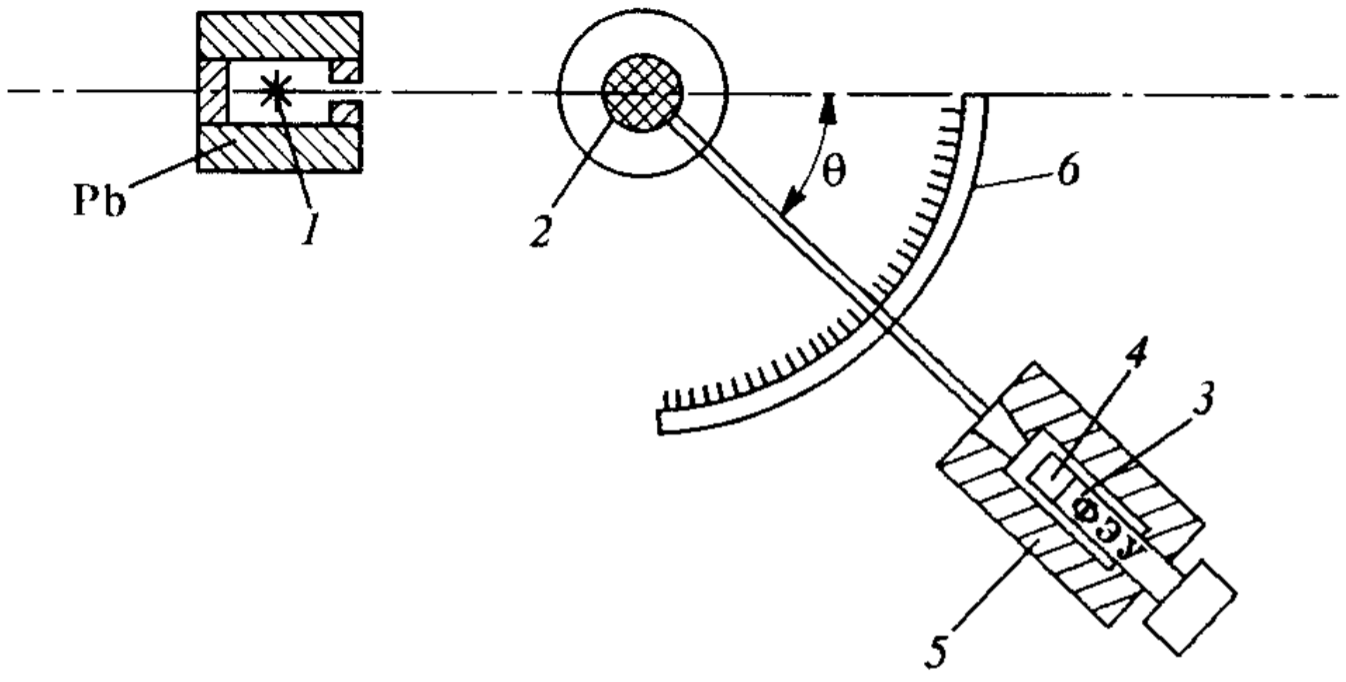
\includegraphics[width=0.5\textwidth]{img/1.png}
      \centering
      \caption{(a) Блок-схема установки по изучению рассения $\gamma$-квантов. (b) Блок-схема измерительного комплекса.}
    \end{figure}
    На Рис. 1а изображена блок-схема установки. 
    Источником (1) служит $^{137} Cs$, испускающий $\gamma$-лучи с энергией $662$ кэВ, который помещён в толстостенный свинцовый контейнер с коллиматором. 
    Сформированный коллиматором узкий пучок $\gamma$-квантов попадает на графитовую мишень (2), испытывает рассеяние и регистрируется сцинтилляционным счётчиком, состоянищим из фотоэлектронного умножителя (ФЭУ) и сцинтиллятора -- выходное окно сцинтиллятора находится в оптическом контакте с фотокатодом ФЭУ. 
    Сигналы, возникающием в аноде ФЭУ, подаются на компьютер для амплитудного анализа. 
    Кристалл и ФЭУ расположены в светонепроницаемом блоке, укреплённого на горизонтальной штанге, которая может вместе с ним вращаться, угол поворота отсчитывается по лимбу (6). 
    Головная часть сцинтилляционного блока закрыта свинцовым коллиматором (5), который формирует входной пучок и защищает детектор от постороннего излучения, в основном $\gamma$-квантов, проходящих через стенки защитного контейнера источника. 
    При больших углах измерения для дополнительной защиты между контейнером и источником и детектором ставился свинцовый экран.
  
  \section{Ход работы}

    В ходе работы были измерены координаты пиков излучения в зависимости от угла рассеяния:
    \begin{table}[h]
      \begin{tabular}{|c|c|c|c|c|c|c|c|c|c|c|c|c|c|}
      \hline
      $\theta^o$          & 0   & 10  & 20  & 30  & 40  & 50  & 60  & 70  & 80  & 90  & 100 & 110 & 120 \\ \hline
      $N_{\text{канала}}$              & 968 & 843 & 852 & 742 & 664 & 583 & 518 & 459 & 414 & 366 & 322 & 303 & 288 \\ \hline
      \end{tabular}
    \end{table}
    При измерении положения пика измерялась координата его оси симметрии.
    В результате этого пристуствует ошибка связанная с дискретностью каналов и с неточностью определения оси симметрии.
    Таким образом примем погрешность данных равной:
    \begin{equation}
      \delta_N \approx 1 \%      
    \end{equation} 
    По полученным данным был построен график зависимости обраьного номера канала от косинуса угла рассеяния:\par
    \begin{figure}[h!]
      \centering
      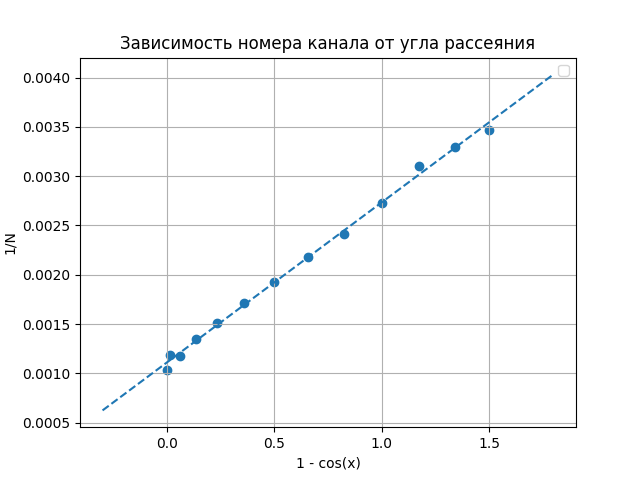
\includegraphics[width=15cm]{img/gra.png}
      \caption{График зависимоти энергии от угла рассеяния}
    \end{figure}\par
    По графику были найдены:
    \begin{equation}
      A = 16.2 * 10^{-4} \hspace{10mm}
      1/N(0) = 11.1 * 10^{-4} \hspace{10mm}
      1/N(90) = 27.3 * 10^{-4}
    \end{equation}
    Погрешность углового коэффициента А примерно 1 \%, поэтому примеем погрешность E равной такому же значению.
    Итогова япогрешность энергии покоя электрона:
    \begin{equation}
      \delta \approx 2 \%
    \end{equation}
    Энергия электронов с учетом погрешности:
    \begin{equation}
      mc^2 = E_\gamma \dfrac{N(90)}{N(0) - N(90)} = 662  \frac{1 / 27.3}{1 / 11.1 - 1 / 27.3} = 453 \pm 9[\text{кэВ}]
    \end{equation}
  \newpage

  \section{Вывод}
    
    Конечная погрешность результатов мала, поэтому из эксперимента можно сделать вывод о том, что эффект Комптона выполняется.\par 
    Табличное значение энергии покоя электронов $mc^2 = 511\text{кэВ}$ больше получившегося значения.
    При измерении пика присутствовал фон, который имел явный наклон близкий к линейному.
    С его учетом реальные значения пиков N должны быть больше.
    Таким образом реальное значение энергии покоя электронов тоже должно быть быольше полученного. 
    
\end{document}